\documentclass[../Thesis.tex]{subfiles}
\begin{document}
	
	\section{State of the Art Review}
	\label{sec:state_of_the_art_review}
	
	Traditional imperative solutions for solving the graph edit distance (GED) problem do exist and can be quite effective for graphs of modest size. These methods typically involve explicit algorithms that compare graphs node by node and edge by edge, often using combinatorial techniques. However, as the number of nodes in the graph increases, the complexity of these methods grows exponentially, leading to scalability issues. In such cases, imperative solutions often become impractical, taking an inordinate amount of time to compute the GED.
	
	To address these scalability challenges, recent research has focused on leveraging artificial intelligence (AI) models. These AI-based approaches offer more robust and scalable solutions by learning patterns and features from graph data, significantly reducing computation times and improving accuracy. In this section, we review some of the prominent AI-based models that have advanced the state of the art in GED computation, including SimGNN, GPN, TaGSim, and GedGNN.
	
	\subsection{SimGNN}

	The first innovative model that significantly outperformed the competition is SimGNN \cite{simgnn__a_neural_network_approach_to_fast_graph_similarity_computation}, introduced in 2019. SimGNN serves as a foundational model in the field of graph similarity computation, and subsequent models often inherit its core concepts, making it the starting point of reference for anyone working in this niche field.
	
	SimGNN is an end-to-end neural network-based approach designed to learn a function that maps a pair of graphs to a similarity score. An overview of SimGNN is illustrated in \autoref{fig:simgnn_architecture}. The architecture of SimGNN involves several key stages:
	
	\begin{itemize}
		\item \textbf{Node Embedding Stage}: Each node in the graph is transformed into a vector that encodes its features and structural properties.
		\item \textbf{Graph-Level Embedding Stage}: The node embeddings are aggregated using an attention mechanism to produce a single embedding for each graph.
		\item \textbf{Graph-Graph Interaction Stage}: The graph-level embeddings of the two graphs are interacted to produce interaction scores that represent the similarity between the graphs.
		\item \textbf{Final Similarity Score Computation Stage}: The interaction scores are further processed to compute the final similarity score, which is compared against the ground-truth similarity score for parameter updates.
	\end{itemize}
	
	In addition to the graph-level embedding interaction strategy, SimGNN incorporates a pairwise node comparison strategy:
	
	\begin{itemize}
		\item \textbf{Pairwise Node Comparison}: This strategy involves computing pairwise interaction scores between the node embeddings of the two graphs. For graphs of different sizes, fake nodes with zero embeddings are added to the smaller graph to ensure compatibility. The resulting similarity matrix is used to extract histogram features, which are then combined with graph-level interaction scores to provide a comprehensive view of graph similarity.
	\end{itemize}
	
	The combination of these two strategies allows SimGNN to capture both coarse global comparison information and fine-grained node-level comparison information, resulting in a robust and thorough approach to graph similarity computation.
	
	\begin{figure}[H]
		\centering
		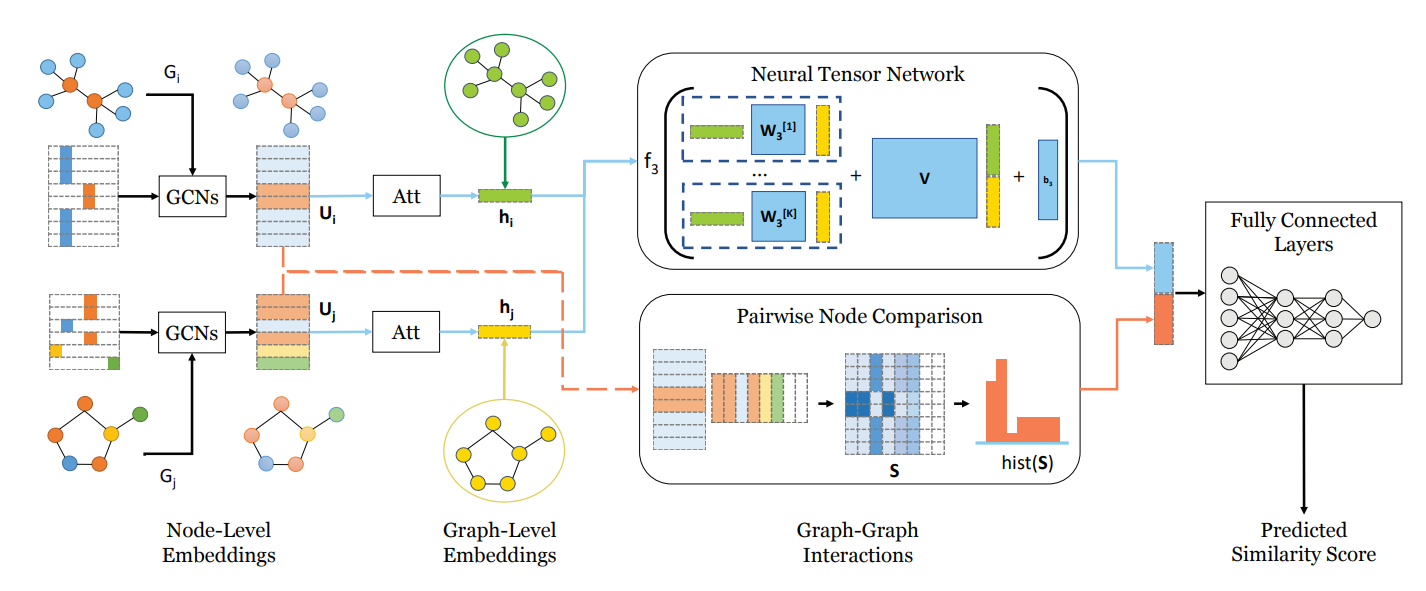
\includegraphics[width=\textwidth]{Images/simgnn_architecture.png}
		\caption{SimGNN architecture overview.}
		\label{fig:simgnn_architecture}
	\end{figure}
	
	\subsection{GedGNN}
	
	Very recently (2023), the GedGNN \cite{computing_graph_edit_distance_via_neural_graph_matching} model introduced significant advancements in the field of graph similarity computation, demonstrating substantial performance improvements over previous models like SimGNN. An overview of GedGNN is illustrated in \autoref{fig:gedgnn_architecture}. The architecture of GedGNN comprises several key components:
	
	\begin{itemize}
		\item \textbf{Node Embedding Generation}: GedGNN employs a Graph Neural Network (GNN) to generate node embeddings for the input graphs. Specifically, it utilizes a three-layer Graph Isomorphism Network (GIN), which is known for its exceptional ability to capture intricate graph structures.
		\item \textbf{Cross Matrix Modules}: GedGNN incorporates two distinct cross matrix modules to capture node-to-node correspondences between the embeddings of the two graphs:
		\begin{itemize}
			\item One module produces a matching matrix ($A_{\text{match}}$), which predicts the ground-truth matching matrix.
			\item The other module generates a cost matrix ($A_{\text{cost}}$), where each element represents the cost of edit operations required to align nodes between the two graphs.
		\end{itemize}
		\item \textbf{Similarity Score Prediction}: The final similarity score, representing the graph edit distance (GED) value, is computed by calculating the weighted sum of costs in the cost matrix, with an additional bias value.
	\end{itemize}
	
	Compared to SimGNN, GedGNN offers several key advancements, including enhanced efficiency, increased accuracy, and greater robustness. Additionally, GedGNN is capable of retrieving an edit path between the two graphs in input. A post-processing algorithm based on \(k\)-best matching is employed to derive \(k\) potential node matchings from the matching matrix produced by GedGNN, with the best matching leading to a high-quality edit path.
	
	\begin{figure}[H]
		\centering
		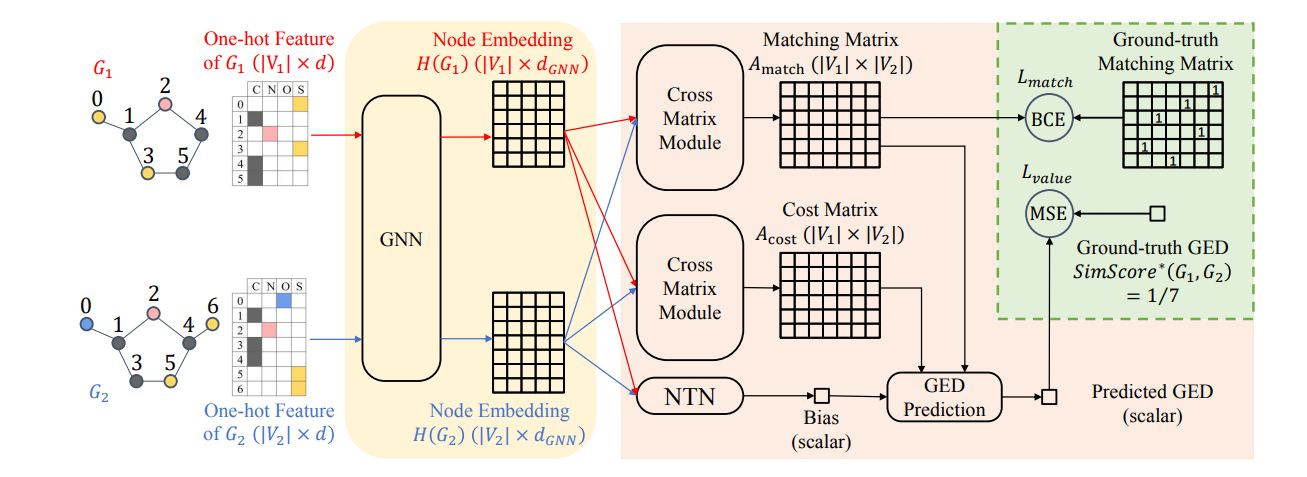
\includegraphics[width=\textwidth]{Images/gedgnn_architecture.png}
		\caption{GedGNN architecture overview.}
		\label{fig:gedgnn_architecture}
	\end{figure}
	
	\subsection{Other Relevant Mentions}
	
	This section highlights additional notable contributions in the field of graph similarity and edit distance computation, showcasing a range of innovative approaches and models.
	
	\begin{itemize}
		
		\item Graph Partitioning and Graph Neural Network Based Hierarchical Graph Matching for Graph Similarity Computation \cite{graph_partitioning_and_graph_neural_network_based_hierarchical_graph_matching_for_graph_similarity_computation} proposes \textbf{PSimGNN}, which partitions graphs and uses a graph neural network for efficient similarity computation, combining coarse and fine-grained approaches to outperform existing methods.
		
		\item NOAH: Neural Optimized A* Search Algorithm for Graph Edit Distance Computation \cite{noah__neural_optimized_a*_search_algorithm_for_graph_edit_distance_computation} proposes \textbf{Noah}, which integrates A* search with Graph Path Networks for approximate GED computation, optimizing search complexity and demonstrating practical effectiveness.
		
		\item Learning Efficient Hash Codes for Fast Graph Based Data Similarity Retrieval \cite{learning_efficient_hash_codes_for_fast_graph_based_data_similarity_retrieval} proposes \textbf{HGNN}, combining GNNs with hash learning for efficient graph-based data retrieval, addressing irregular structures and high computational complexity in graph operations.
		
		\item More Interpretable Graph Similarity Computation via Maximum Common Subgraph Inference \cite{more_interpretable_graph_similarity_computation_via_maximum_common_subgraph_inference} proposes \textbf{INFMCS}, an interpretable model inferring Maximum Common Subgraph during graph similarity learning, combining transformers and graph convolution for improved performance.
		
		\item H2MN: Graph Similarity Learning with Hierarchical Hypergraph Matching Networks \cite{h2mn__graph_similarity_learning_with_hierarchical_hypergraph_matching_networks} proposes \textbf{H2MN}, leveraging hierarchical hypergraph matching for graph similarity learning, employing hyperedge pooling and multi-perspective matching to achieve superior results.
		
		\item Efficient Graph Edit Distance Computation using Isomorphic Vertices \cite{efficient_graph_edit_distance_computation_using_isomorphic_vertices} proposes \textbf{Isomorphic Vertex Reduction}, a method to reduce GED computation costs by addressing redundant mappings from isomorphic vertices, aiming for optimization in exact and approximate GED computations.
		
		\item Exploring Attention Mechanism for Graph Similarity Learning \cite{exploring_attention_mechanism_for_graph_similarity_learning} proposes \textbf{NA-GSL}, a unified framework incorporating attention mechanisms for graph similarity estimation, achieving improved performance through graph convolution and cross-graph co-attention.
		
		\item Graph Edit Distance Learning via Different Attention \cite{graph_edit_distance_learning_via_different_attention} proposes \textbf{DiffAtt}, a graph-level fusion module leveraging attention mechanisms to compute GED efficiently, outperforming traditional methods in accuracy and speed.
		
		\item Graph-Graph Context Dependency Attention for Graph Edit Distance \cite{graph_graph_context_dependency_attention_for_graph_edit_distance} proposes \textbf{GED-CDA}, incorporating context dependency attention modules for GED computation, capturing inter- and intra-graph dependencies effectively, and demonstrating high efficiency.
		
		\item GREED: A Neural Framework for Learning Graph Distance Functions \cite{greed__a_neural_framework_for_learning_graph_distance_functions} proposes \textbf{GREED}, a siamese GNN model for GED and Subgraph Edit Distance, preserving metric properties and achieving high accuracy and efficiency for large-scale retrieval tasks.
		
		\item MATA: Combining Learnable Node Matching with A* Algorithm for Approximate Graph Edit Distance \cite{mata_combining_learnable_node_matching_with_a*_algorithm_for_approximate_graph_edit_distance} proposes \textbf{MATA*}, a hybrid model combining GNNs and A* algorithms for approximate GED computation, addressing scalability and efficiency issues with promising results.
		
		\item Multilevel Graph Matching Networks for Deep Graph Similarity Learning \cite{multilevel_graph_matching_networks_for_deep_graph_similarity_learning} proposes \textbf{MGMN}, a multilevel graph matching network capturing cross-level interactions for graph similarity, demonstrating superior performance and robustness with increasing graph size.
		
		\item Wasserstein Graph Distance Based on L1-Approximated Tree Edit Distance Between Weisfeiler-Lehman Subtrees \cite{wasserstein_graph_distance_based_on_l1_approximated_tree_edit_distance_between_weisfeiler_lehman_subtrees} proposes \textbf{WWLS}, combining Wasserstein distance with L1-approximated tree edit distance to detect subtle structural differences, showing superior performance in graph classification tasks.
		
		\item EUGENE: Explainable Unsupervised Approximation of Graph Edit Distance \cite{eugene__explainable_unsupervised_approximation_of_graph_edit_distance} proposes \textbf{EUGENE}, an unsupervised method for GED estimation using algebraic representation and rounding, demonstrating competitive performance and potential for broader applications.
	\end{itemize}
	
	
\end{document}
